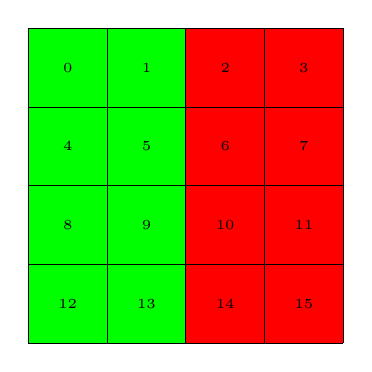
\begin{tikzpicture}[font=\tiny,
  every node/.style={minimum size=1cm-\pgflinewidth, outer sep=0pt}]
  %% https://tex.stackexchange.com/questions/274219/drawing-a-multicolored-grid-using-tikz
  %% draw gird
  \draw[step=1cm, color=black, line width=0.5pt] (0,0) grid (4,4);
  %% put in colors
  % First row
  \node[fill=green] at (0.5, +3.5) {0};
  \node[fill=green] at (1.5, +3.5) {1};
  \node[fill=red] at   (2.5, +3.5) {2};
  \node[fill=red] at   (3.5, +3.5) {3};
  % Second row
  \node[fill=green] at (0.5, +2.5) {4};
  \node[fill=green] at (1.5, +2.5) {5};
  \node[fill=red] at   (2.5, +2.5) {6};
  \node[fill=red] at   (3.5, +2.5) {7};
  % Third row
  \node[fill=green] at (0.5, +1.5) {8};
  \node[fill=green] at (1.5, +1.5) {9};
  \node[fill=red] at   (2.5, +1.5) {10};
  \node[fill=red] at   (3.5, +1.5) {11};
  % Fourth row
  \node[fill=green] at (0.5, +0.5) {12};
  \node[fill=green] at (1.5, +0.5) {13};
  \node[fill=red] at   (2.5, +0.5) {14};
  \node[fill=red] at   (3.5, +0.5) {15};
\end{tikzpicture}
%%
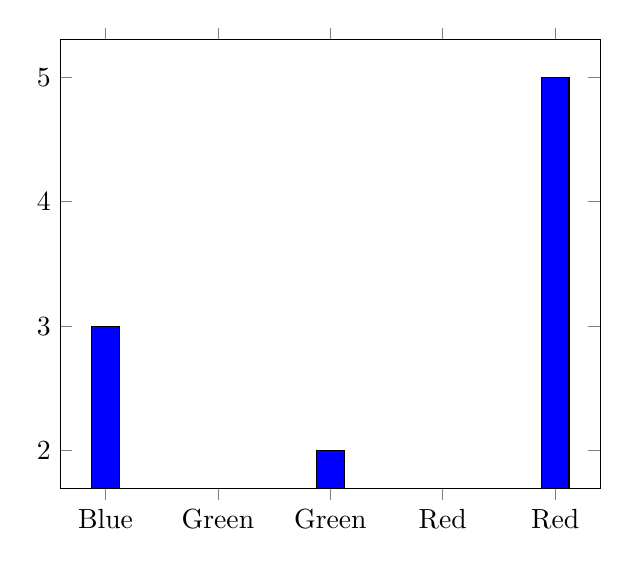
\begin{tikzpicture}
  \begin{axis}[ybar,
      symbolic x coords={Blue, Green, Red},
      enlargelimits=true
    ]
  \addplot [draw, fill=blue] coordinates {
    (Red, 5)
    (Blue, 3)
    (Green, 2)
    };
\end{axis}
\end{tikzpicture}
%%

